Sea  $\Omega' \subset \mathbb{R}^3$ el dominio de inter\'es, $t_f>0$ el tiempo final de la simulaci\'on,   $\vec v : [0,t_f]\times \Omega \rightarrow  \mathbb{R}^3$ el campo de velocidad, y $p : [0,t_f] \times \Omega \rightarrow \mathbb{R}$ el campo de presiones, luego las ecuaciones de Navier-Stokes para un fluido incompresible con densidad $\rho \in \mathbb{R}^+$, superficie libre  $\eta: [0,t_f] \times \Omega \rightarrow \mathbb{R}$ sobre un fondo (topograf\'ia-batimetr\'ia) de forma dada por $b:\Omega \rightarrow \mathbb{R}$, sujeto a fuerzas por uindad de volumen $\vec f_b : \Omega \rightarrow \mathbb{R}^3$,  cuando se desprecian efectos disipativos, son \cite{toro}
\begin{align}
  \begin{split}
    \nabla \cdot \vec v &= 0 \\
    \frac{\partial }{\partial t}\vec v + \nabla \cdot \vec v \otimes \vec v  &= -\frac{1}{\rho}\nabla p + \vec f_b    \\
    v_3|_{z=\eta	} &= \frac{\partial \eta}{\partial t}+(\vec v \cdot \nabla )\eta \\
    v_3|_{z=b} &= \frac{\partial b}{\partial t} + (\vec v \cdot \nabla )b \\    
    p|_{z = \eta} &= 0
  \end{split}  
  \label{NS-incompresible}
\end{align}

Bajo el supuesto que las ondas son suficietemente largas es posible asumir que no existen aceleraciones verticales, y por medio de integraci\'on vertical entre el fondo $b$ y la superficie libre $\eta$, las Ecuaciones No Lineales de Aguas Someras (Non-Linear Shallow water Equations, NSWE) son, para una bah\'ia con borde impermeable $\partial\Omega_h$ y linea nodal $\Omega_g$ tales que $\partial \Omega = \partial \Omega_h \cup \partial \Omega_g$,

\begin{equation}  \begin{split}
\left(\eta\right)_{t}+\left(hu\right)_{x}+\left(hv\right)_{y} & =0  \text{       si } x \in \Omega\\
  \left(hu\right)_{t}+(hu^{2}+\frac{1}{2}gh^{2})_{x}+(huv)_{y} & =-ghb_{x}  \text{   si } x\in\Omega\\
  \left(hu\right)_{t}+(huv)_{x}+(hv^{2}+\frac{1}{2}gh^{2})_{y} & =-ghb_{y}  \text{     si } x \in \Omega\\
  (hu,hv) \cdot \vec n &= 0  \text{ si    } x\in\partial \Omega_h \\
   \eta &= 0  \text{ si    } x \in \partial \Omega_g  
  \end{split}
  \label{eq:nswe_cart}
  \end{equation}

 Donde, siguiendo la figura \ref{fig:vars}, $h(t,x,y)=\eta(t,x,y)-b(x,y) \geq 0$ es la altura de la columna de agua,  y $(u,v)$ las componentes de velocidad horizontal promediadas en la vertical, dadas por
 $$
  (u,v)=\frac{1}{h}\int_{b}^\eta (v_1,v_2)dz
 $$
  
  \begin{figure}
    \centering
    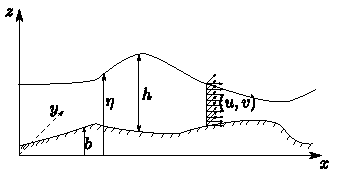
\includegraphics[width=10cm]{figs/variables.pdf}    
    \caption{Schematic view of hydrodynamic variables defined for the Non-Linear Shallow Water Equations.}
    \label{fig:vars}
  \end{figure}

Las ecuaciones en \eqref{eq:nswe_cart}, forman un sistema hiperbo\'olico no lineal de ecuaciones diferenciales parciales. Sin embargo, si se consideran peque\~nas perturbaciones a una masa de agua en reposo, es decir
$$
	\eta=h+\eta' \hspace{.5cm} u=0+u',\hspace{.5cm} v = 0 + v'
$$
donde la notaci\'on $f'$ indica peque\~nas perturbaciones sobre $f$, y $h:\Omega\rightarrow \mathbb{R}$ se deduce las ecuaciones lineales de aguas someras, donde es posible asumir que $h$ no depende del tiempo pero s\'i del espacio

\begin{align}
	\begin{split}
	\frac{\partial \eta'}{\partial t}+\frac{\partial hu'}{\partial x}+\frac{\partial hv'}{\partial y} = 0  \text{ si } x \in \Omega\\
    \frac{\partial u'}{\partial t} + g\frac{\partial \eta}{\partial x}=0  \text{ si } x \in \Omega\\
    \frac{\partial v}{\partial t} + g\frac{\partial \eta}{\partial y} = 0  \text{ si } x \in \Omega \\
    (hu',hv') \cdot \vec n = 0 & \text{ si } x\in\partial \Omega_h \\
   \eta' = 0  \text{ si } x \in \partial \Omega_g  
    \end{split}
    \label{swe}
\end{align}

    Si pedimos que la segunda derivada temporal de $\eta',u',v'$ sea continua, y multiplicamos la segunda y tercera ecuaci\'on de \eqref{swe}, por $h$ y derivamos respecto a $x$ e $y$ entonces se cumple que 
    \begin{equation}
    	\begin{split}
    	\frac{\partial^2 \eta}{\partial t^2} - \nabla \cdot( gh \nabla \eta) = 0, \text{ si } x \in \Omega \\
        \frac{\partial \eta}{\partial \vec n} = 0 \text{ si } x \in \partial \Omega_h \\
        \eta = 0 \text{ si }x \in \partial \Omega_g
        \end{split}
     \label{eqonda}
    \end{equation}

	Finalmente, si se estudian ondas estacionarias, es posible separar variables y escribir (abusando de notaci\'on en $u$), con $u:\Omega \rightarrow \mathbb{R}$
    \begin{equation}
    	\eta(t,x,y) =Re\left\{ u(x,y) e^{-i\Omega t}\right\}
    \end{equation}
    
    lo cual, sustituyendo en \ref{eqonda} conduce a 
    
    \begin{equation}
    	\nabla \cdot gh \nabla u + \omega^2 u = 0 \text{ si } x \in \partial \Omega\\
        \frac{\partial u}{\partial \vec n} = 0 \text{ si } x \in \partial \Omega_h \\
        u = 0 \text{ si } x \in \partial \Omega_g
        \label{helmholtz}
    \end{equation}
    
    
    